% Created 2016-04-27 Wed 13:09
\documentclass[10pt,t,a4paper]{article}
\usepackage[utf8]{inputenc}
\usepackage[T1]{fontenc}
\usepackage{fixltx2e}
\usepackage{graphicx}
\usepackage{grffile}
\usepackage{longtable}
\usepackage{wrapfig}
\usepackage{rotating}
\usepackage[normalem]{ulem}
\usepackage{amsmath}
\usepackage{textcomp}
\usepackage{amssymb}
\usepackage{capt-of}
\usepackage{hyperref}
\author{Mikael Svahnberg\thanks{Mikael.Svahnberg@bth.se}}
\date{2016-04-27}
\title{Packages and their Dependencies}
\hypersetup{
 pdfauthor={Mikael Svahnberg},
 pdftitle={Packages and their Dependencies},
 pdfkeywords={},
 pdfsubject={},
 pdfcreator={Emacs 25.1.50.1 (Org mode 8.3.4)}, 
 pdflang={English}}
\begin{document}

\maketitle

\section{Introduction}
\label{sec:orgheadline1}
I received a question:

\begin{quote}
Hej! Vår grupp har stött på ett problem med Uppgift 2, kapitel 2.2: Packages and their relations/dependencies.
Vi vet inte riktigt vad som ska göras här och vore tacksamma om vi fick ett exempel.
\end{quote}

This made me realise that this is an aspect that I have not covered in the course. Packages are covered in chapter 31.18 in the course book (with some guidelines for how to think when creating packages in chapter 35.1), but here is the TL;DR of them.

\section{What are Packages?}
\label{sec:orgheadline6}
A package is a means to hide lower-level details. For example, even if you model each sub-system in your application on a separate page, you will then need to have an overview of how your separate pages fit together. When you do architectural design (in another course), you will (for one of the views of your system, the Module View) use packages to illustrate how components are implemented as one or a small set of packages.

You can also use them to illustrate that some classes (or other packages) logically ``belong together''. If we look at the Dictionary example discussed in lecture 07 (From Design to Code), we can use three high-level packages to illustrate that we have a Model, Views, and a Controller. In this simple example, there are only a few classes in each, but in a more complex system, you may have quite a number of collaborating classes in each package.

The notation is simply a folder, and this is the analogy as well -- that it is a folder where you may hide stuff. You would typically use this ``hide-the-inside''-mode when you are showing a high-level view of the system. Later on, you would have to open the folder and display the insides as well.

\subsection{Example: Package of Packages\hfill{}\textsc{Example}}
\label{sec:orgheadline2}
In this example, I am -- on a very high level -- modelling the model, view, and controller packages of the Dictionary system.

I have added dependencies between the packages as well. \emph{Please Note} the direction of the dependency arrow! In this example, \emph{View} depends on \emph{Controller}, and \emph{Controller} depends on the \emph{Model} package.

Source (plantuml) and Diagram:
\begin{verbatim}
@startuml
left to right direction
package Dictionary  {
package Model
package View
package Controller
Model <.. Controller
Controller <.. View
}
@enduml
\end{verbatim}

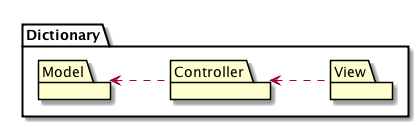
\includegraphics[width=.9\linewidth]{FPackageNotation.png}

\subsection{Example: Package of Classes\hfill{}\textsc{Example}}
\label{sec:orgheadline3}

A first look inside the \emph{View} Package:

Source and Diagram:
\begin{verbatim}
@startuml
Package View {
interface DictionaryView
DictionaryView : +setController(ControllerInterface theController)

DictionaryView <|-- WordView
DictionaryView <|-- WordDefinitionView
DictionaryView <|-- LogView
}
@enduml
\end{verbatim}

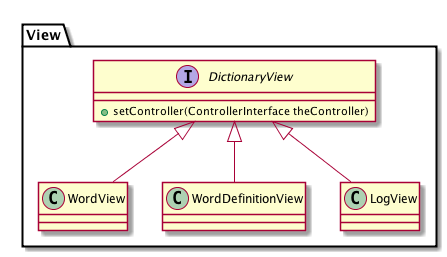
\includegraphics[width=.9\linewidth]{FPackageOfClasses.png}

\subsection{Example: Referring to elements from another package\hfill{}\textsc{Example}}
\label{sec:orgheadline4}
A package ``owns'' everything that is inside the package. This means that if we want to refer to something from another package, we need to have a way to ``import'' it -- or link directly across package borders. Both are possible, but the ``import'' facility is preferred since it leads to a less cluttered diagram. This is done using the \emph{scope} operator from C++: \texttt{Package::Class} .

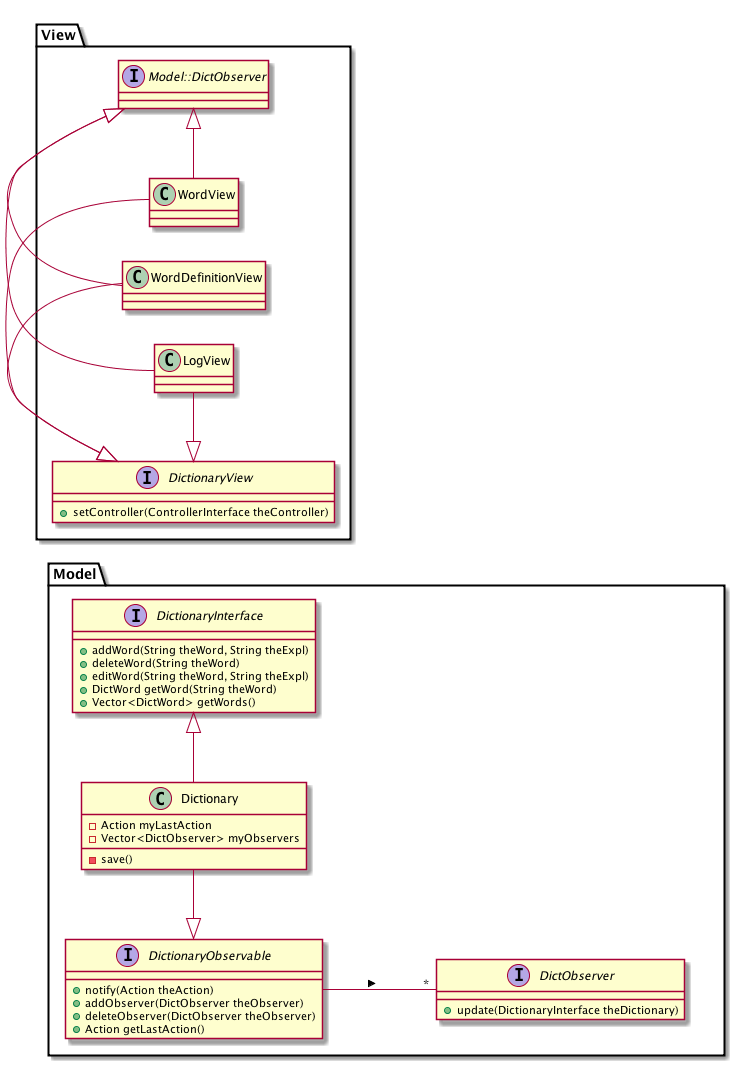
\includegraphics[width=.9\linewidth]{FPackageCrossRef.png}

\subsection{One More Example: Pacman\hfill{}\textsc{Example}}
\label{sec:orgheadline5}
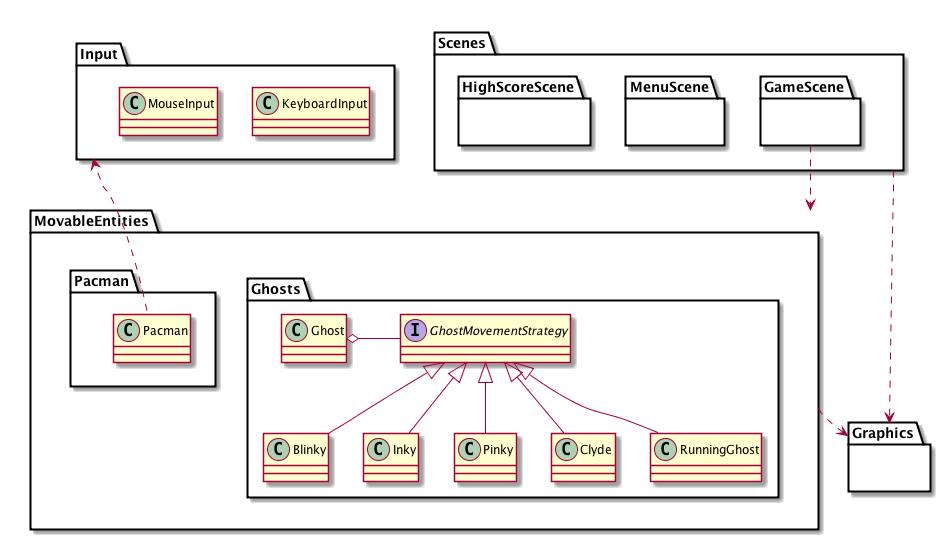
\includegraphics[width=.9\linewidth]{FPackagesPacman.png}
\end{document}